%Gebruik van stylesheets term in het nederlands: http://www.bol.com/nl/p/websites-opmaken-met-css/1001004010718921/
%OPMERKING:  het gebruik van 'CSS-stylesheets' slaat op niets (kijk naar de betekenis van CSS :-))
%OPMERKING: is het UI-elementen of UI elementen idem voor HTML5-code of HTML5 code?

\chapter{Literatuurstudie}
\label{hoofdstuk:2}
Eerst zullen we kijken naar welke mobiele apparaten er allemaal bestaan (\ref{sec:mobiele-apparaten}). Vervolgens zullen we kijken wat er onder de motorkap van deze apparaten zit, namelijk welke mobiele besturingssystemen (\ref{sec:mobiele-besturingssystemen}), welke mobiele applicaties (\ref{sec:mobiele-applicaties}) en welke mobiele webbrowsers (\ref{sec:mobiele-webbrowsers}) er bestaan. Daarna zullen we het hebben over de drie bouwblokken van het web (\ref{sec:html5-css3-js}):  HTML,  CSS en JavaScript. Hierna zullen we het hebben over mobiele HTML5 raamwerken (\ref{sec:mobiele-html5-raamwerken}).  Ten slotte kijken we naar verschillende manieren over hoe we een raamwerk kunnen vergelijken (\ref{sec:vergelijken-raamwerken}).

%%%%%%%%%%%%%%%%%%%%%%%%%%%%%%%%%%%%%%%%%%%%%%%%%%%%%%%%%%%%%%%%%%
%%%%%%%%%%%%%%%%%%%%%%%%%%%%%%%%%%%%%%%%%%%%%%%%%%%%%%%%%%%%%%%%%%

\section{Mobiele apparaten}
\label{sec:mobiele-apparaten}
Mobiele apparaten vind je in alle soorten en maten, met weinig of veel opties, voor weinig of veel geld. Het verdient daarom aandacht om deze diversiteit onder de loep te nemen. Eerst zullen we de soorten mobiele apparaten bekijken. Daarna zullen we ingaan op de kenmerken.

\subsection{Soorten}
Sinds de voorstelling van de Apple iPhone in 2007~\cite{David2011}, stijgt het gebruik van de \term{smartphone} ontzettend snel in onze samenleving.  Momenteel zijn er al meer dan 1 miljard toestellen in gebruik~\cite{Yang2012}! Foto's of video's nemen, navigeren naar het dichtstbijzijnde restaurant of nog snel het weer van de komende dagen opzoeken, het is allemaal mogelijk. Hoewel Apple de lat hoog heeft gelegd met het uitbrengen van de iPhone, zijn er ook nog andere spelers op de markt. Zo hebben we bijvoorbeeld ook de op Google's Android gebaseerde \term{smartphones} zoals de Nexus 4 en de op Windows Phone gebaseerde \term{smartphones} zoals de Nokia Lumia 800.

Niet enkel de \term{smartphone}	 behoort tot de categorie van mobiele apparaten, maar ook de \term{tablet}. Ook hier kan terug gedacht worden aan één van Apple's succesvolle producten, namelijk de in 2010 uitgebrachte iPad. Er dient echter wel opgemerkt te worden dat tien jaar voordien, Microsoft al eerder een \term{tablet} uitbracht met veel minder succes.

De \term{e-reader} behoort tot de laatste categorie van mobiele apparaten. Deze wordt hoofdzakelijk gebruikt om digitale boeken te lezen, maar betere modellen laten bijvoorbeeld ook toe om te surfen op het internet. Ook hier bestaat er een variëteit aan modellen zoals de Kindle van Amazon en de Reader van Sony.

\subsection{Kenmerken}
Door de vele verschillende soorten en modellen aan mobiele apparaten, is het nodig om op een hoog niveau te bekijken over welke kenmerken deze allemaal (kunnen) beschikken. Bij deze bespreking zullen we enkel ingaan op de kenmerken van \term{smartphones} en \term{tablets}. Sommige kenmerken kunnen ook van toepassing zijn op \term{e-readers}. Deze kenmerken zijn gebaseerd op~\cite{PhilDutson2012}.
%TODO sommige eruit halen

\subsubsection{Resolutie en PPI}
Een eerste kenmerk, waar vooral Apple met haar Retina graag mee uitpakt, is de resolutie. Dit is het aantal pixels getoond op het beeldscherm en wordt uitgedrukt in breedte $\times$ hoogte. Hoe kleiner, hoe minder er op het scherm kan worden getoond. Dit is vooral belangrijk wanneer veel informatie op het scherm wordt getoond. Indien men maar over een kleine resolutie beschikt, zal men moet scrollen om te rest van de informatie te kunnen zien.

Als men naast de resolutie ook nog eens gaat rekening houden met de fysieke grootte van het scherm, dan kunnen we spreken van over pixels per inch of kortweg PPI. De eerste iPhone had een resolutie van 320$\times$480 en een 3,5” scherm, wat neerkomt op 163 PPI. De iPhone4 (Retina) daarentegen heeft een resolutie van 640$\times$960 en een 3,5” scherm, wat neerkomt op 326 PPI. Met andere woorden zijn er meer pixels op dezelfde fysieke grootte geplaatst, wat een scherper beeld tot resultaat heeft.

Een overzicht van vaak voorkomende resoluties voor mobiele apparaten wordt getoond op de figuur \ref{fig:resoluties}.

% TODO afbeelding misschien vectorieel maken:  
%Sander: nieuwe recente afbeelding gebruiken ;)
\begin{figure}
  \centering
  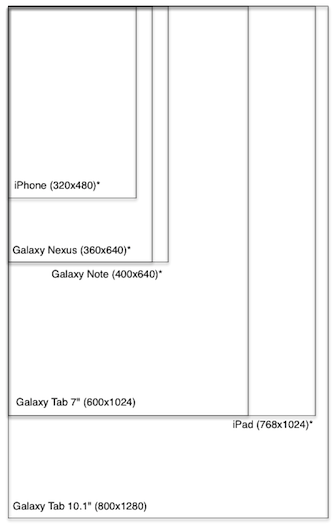
\includegraphics[height=0.8\textwidth]{figuren/mobile-devices-resolutions.png}
  \caption{Resoluties van bekende mobiele apparaten~\cite{Wolfermann2012}.}
  \label{fig:resoluties}
\end{figure}

\subsubsection{Aanraakscherm}
De meest voorkomende soorten schermen zijn resistieve en capacitieve aanraakschermen. De eerste soort maakt gebruik van twee lagen die gescheiden worden door een tussenruimte. Door druk ontstaat er contact tussen de twee lagen. Meestal wordt bij deze soort schermen een stylus meegeleverd. 

De tweede soort maakt gebruik van veranderingen in frequentie. Door het scherm aan te raken met je vinger, dat een geleider is, ontstaat er een kleine verandering in frequentie die gedetecteerd wordt. Niet-geleidende materialen zullen geen frequentieverandering veroorzaken, wat verklaart dat zo'n scherm niet reageert als je het aanraakt met een handschoen.

% \subsubsection{Oriëntatie}
% Een handig kenmerk is dat vele mobiele apparaten kunnen detecteren hoe ze gehouden worden door de gebruiker. Dit maakt het mogelijk om de informatie zo optimaal mogelijk op het scherm te tonen. Men kan bijvoorbeeld een verschillende lay-out voorzien voor een staand en liggend scherm.
% 
% \subsubsection{Versnellingsmeter}
% Als het mobiele apparaat een versnellingsmeter bevat, is het mogelijk om hiervan in spelletjes e.d. gebruik van te maken.
% 
% \subsubsection{Afstandssensor}
% Niet veel mobiele apparaten beschikken over dit kenmerk, maar dit kan bijvoorbeeld gebruikt worden wanneer een gebruiker met zijn smartphone aan het bellen is, waarbij het scherm zichzelf automatisch uitschakelt als het tegen de wang wordt gehouden.

% \subsubsection{Fysiek toetsenbord}
% Sommige apparaten beschikken ook nog over een fysiek toetsenbord, soms ook in combinatie met een aanraakscherm. 
%TODO Sander:  Als er in de tekst naar kenmerken van een device wordt verwezen krijg je altijd het voorbeeld GPS of Camera.  Dat lijken mij ook de twee belangrijkste voor POC.  Deze twee zijn mss voldoende om dan te bespreken?

\subsubsection{GPS}
Een kenmerk die heel handig is, is het \term{global positioning system} of kortweg de GPS. Hiermee kan de gebruiker zijn locatie opvragen en doorgeven aan een applicatie om zo bijvoorbeeld het dichtstbijzijnde restaurant te vinden. Doordat het soms wat kan duren vooraleer de locatie is vastgesteld, kunnen sommige mobiele apparaten ook gebruik maken van mobiele masten om zo, hetzij minder nauwkeurig, sneller de locatie te bepalen.

% \subsubsection{Barometer}
% Sommige mobiele apparaten zijn uitgerust met een barometer. Naast het meten van de druk die kan helpen bij het bepalen van het weer, helpt deze de GPS bij het bepalen van de locatie.

\subsubsection{Camera}
Vele mobiele apparaten zijn uitgerust met een camera. Sommige bevatten zelfs twee camera's. De camera vooraan is meestal van mindere kwaliteit is en wordt gebruikt om bijvoorbeeld videogesprekken te voeren. Achteraan zit meestal een betere camera om mooie kiekjes te kunnen nemen.

Daarnaast kan de camera ook gebruikt worden voor toegevoegde realiteit (TR) of  \term{augmented reality} (AR). Hiermee kunnen dingen worden toegevoegd aan het beeld dat door de camera werd geregistreerd.

Een andere toepassing van de camera is het inscannen van barcodes. De populaire QR-code kan worden gebruikt om tekst in op te slaan, een link naar een website te tonen, een telefoonnummer, enz. De gebruiker kan deze code inscannen en zien wat ze betekent.

\subsubsection{Verbinding}
%TODO: Wifi, 3G, EDGE
In deze periode is het ondenkbaar om niet verbonden te zijn met het Internet. Het mobiel apparaat kan meerdere mogelijkheden voorzien om verbinding te maken. Enerzijds kan men verbinden via Wi-Fi. Daarnaast zijn er ook nog andere technologieën zoals 3G mogelijk.

%%%%%%%%%%%%%%%%%%%%%%%%%%%%%%%%%%%%%%%%%%%%%%%%%%%%%%%%%%%%%%%%%%
%%%%%%%%%%%%%%%%%%%%%%%%%%%%%%%%%%%%%%%%%%%%%%%%%%%%%%%%%%%%%%%%%%

\section{Mobiele besturingssystemen}
\label{sec:mobiele-besturingssystemen}
Net zoals er brede waaier bestaat aan besturingssystemen voor personal computers, geldt dit ook zo voor mobiele apparaten. We geven hier een overzicht van mobiele besturingssystemen met een significant marktaandeel~\cite{David2011, Hales2012} zoals iOS en Android, maar ook een nieuwkomer op de markt, namelijk Windows Phone.

\subsection{iOS}
Het iPhone besturingssysteem is voor het eerst uitgekomen in juni 2007 tezamen met de iPhone. Later werd het hernoemd naar iPhone OS en uiteindelijk werd het iOS. Het is duidelijk dat iOS gebonden is aan de hardware van Apple. Verschillende versies volgden elkaar op: iOS 2 (juli 2008), iOS 3 (juni 2009), iOS 4 (juni 2010) en iOS 5 (oktober 2011)~\cite{Deitel2012, PhilDutson2012}. 

De nieuwste versie, iOS 6, werd uitgegeven in september 2012. Nieuwigheden zijn onder andere hun eigen Maps (in plaats van Google Maps) en een Pass Kit (de vervanging van het traditionele trein-, cinematicket, enz.). Daarnaast zijn er ook ander andere verbeteringen uitgevoerd met betrekking tot sociale media en spraakcommando's~\cite{Deitel2012}.

Op figuur \ref{fig:marketshare-ios} is te zien dat bijna twee derde van de iOS-gebruikers al iOS 6 gebruikt.

\begin{figure}
  \centering
  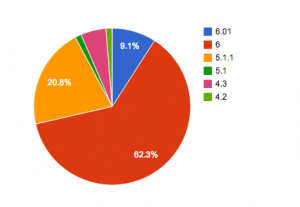
\includegraphics[width=0.5\textwidth]{figuren/marketshare-ios-2012-11-14.png}
  \caption{Marktaandeel iOS-besturingssystemen op 14 november 2012~\cite{Sylvain2012}.}
  \label{fig:marketshare-ios}
\end{figure}

Browsen op het web gebeurt met de geïnstalleerde Mobile Safari webbrowser (zie \ref{sec:mobile-safari}). Applicaties kunnen gedownload worden in de App Store, die sinds iOS 2 aanwezig is~\cite{Deitel2012}. 

\subsection{Android}
Android Inc. werd opgericht in 2003 en werd in 2005 overgekocht door Google Inc~\cite{Satyesh2012}. Het is net zoals iOS een mobiel besturingssysteem, maar in tegenstelling tot iOS is het open~\cite{David2011}. De eerste stabiele versie, Android 1.0, kwam uit in september 2008. Ook hier volgden verschillende versies elkaar op: Android 2.0 (oktober 2009), Android 3.0 (februari 2011) en Android 4.0 (oktober 2011)~\cite{Satyesh2012}. Hun nieuwste versie, Android 4.2, werd aangekondigd in oktober 2012~\cite{Sawers2012}. 

Op figuur \ref{fig:marketshare-android} is het marktaandeel te zien van de verschillende Android besturingssystemen, waargenomen over een periode van 14 dagen. Het is duidelijk dat Gingerbread (Android 2.3) meer dan de helft van het marktaandeel inneemt.
Applicaties worden gedownload in Google Play. Android bevat ook een standaard browser (zie \ref{sec:android-browser}).

\begin{figure}
  \centering
  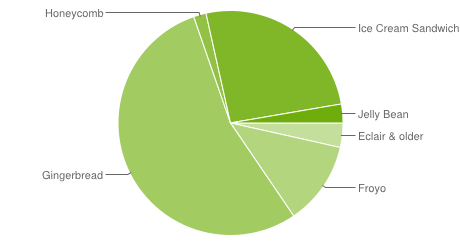
\includegraphics[width=0.7\textwidth]{figuren/marketshare-android-2012-11-01.png}
  \caption{Marktaandeel Android besturingssystemen op 1 november 2012~\cite{Android2012}.}
  \label{fig:marketshare-android}
\end{figure}

\subsection{Windows Phone}
Windows Phone van Microsoft werd aangekondigd in oktober 2010 als vervanging voor Windows Mobile~\cite{Seitz2010,Lieberman2010}. Dit is duidelijk te zien als we kijken naar de versies: de laatste versie was Windows Mobile 6.5.3 en de eerste versie is Windows Phone 7. In 2011 ging Microsoft een partnerovereenkomst aan met Nokia om zo snel de markt te kunnen overwinnen~\cite{Microsoft2011}. De nieuwste versie, Windows Phone 8, werd aangekondigd in oktober 2012~\cite{Reed2012}. 

%%%%%%%%%%%%%%%%%%%%%%%%%%%%%%%%%%%%%%%%%%%%%%%%%%%%%%%%%%%%%%%%%%
%%%%%%%%%%%%%%%%%%%%%%%%%%%%%%%%%%%%%%%%%%%%%%%%%%%%%%%%%%%%%%%%%%

\section{Mobiele applicaties}
\label{sec:mobiele-applicaties}
%TODO Sander: eventueel eerst voorstellen,  dan een paragraafje minivergelijking..
Er zijn drie mogelijkheden om mobiele applicaties te maken~\cite{Accenture2012,Hales2012}. Eén aanpak is het maken van een webapplicatie. Zo'n applicatie wordt geopend vanuit de webbrowser. Een andere aanpak is een native applicatie. Hierbij zal de gebruiker de applicatie installeren op zijn apparaat. Als laatste kan een mix van de vorige gemaakt worden en dat wordt een hybride applicatie genoemd.

\subsection{Webapplicaties}
In het rapport 'The (Not So) Future Web'~\cite{Phifer2011} uit juni 2011 wordt gesteld dat tegen 2015 60\% van alle mobiele bedrijfsapplicaties en 40\% van alle mobiele consumentenapplicaties, webapplicaties zullen zijn. Er zijn namelijk veel voordelen~\cite{Accenture2012} verbonden aan webapplicaties.

Ten eerste heeft iedereen die een webbrowser heeft op zijn mobiel apparaat, toegang tot de applicatie.  Dit voordeel gaat niet op voor een native applicatie dat enkel voor een specifiek platform is geschreven. 

Ten tweede, aansluitend bij het bovenstaande voordeel, moet de code slechts eenmaal worden geschreven. Een vaak voorkomende term die dit samenvat is WORA: \term{write once, run anywhere}~\cite{Hales2012}. Dit is in tegenstelling tot een native applicatie die specifiek geschreven is voor bijvoorbeeld iOS, Android en Windows Phone. Daar dient de code driemaal te worden geschreven \'en te worden onderhouden.

Ten derde moeten webapplicaties niet worden geverifieerd vooraleer ze worden uitgebracht. Dit is wel zo bij native applicaties. Hierdoor kan in een webapplicatie een belangrijke update snel doorgevoerd worden, terwijl de native applicatie nogmaals het verificatieproces moet doorlopen.

\subsection{Native applicaties}
Een andere mogelijk is om een native applicatie te schrijven. Voordelen~\cite{Accenture2012} hier zijn onder meer de snelheidswinst doordat de applicatie rechtstreeks met het besturingssysteem kan werken. Aansluitend bij het vorige kan ook worden geargumenteerd dat het over het algemeen een native applicatie gemakkelijker de kenmerken van het mobiel apparaat, zoals de camera of GPS, aan kan spreken. Ten derde blijft beveiliging nog altijd een knelpunt bij webapplicaties. Een native applicatie heeft hier minder problemen. Als laatste kan opgemerkt worden dat het gebruik van een winkel (\term{store}) voor het aanbieden van een applicatie als voordeel kan gezien worden, afgezien van het verificatieproces. De applicatiewinkel zorgt namelijk voor reclame en correcte uitbetaling bij gebruik van de applicatie.

\subsection{Hybride applicaties}
Er bestaat een mix tussen de twee voorgaande soorten van mobiele applicaties, namelijk een hybride applicatie~\cite{Accenture2012}. Hierbij wordt de webapplicatie verpakt in een native applicatie. Hierdoor kan men specifieke kenmerken van het mobiel apparaat benaderen die men vanuit een pure webapplicatie niet kon benaderen.

%%%%%%%%%%%%%%%%%%%%%%%%%%%%%%%%%%%%%%%%%%%%%%%%%%%%%%%%%%%%%%%%%%
%%%%%%%%%%%%%%%%%%%%%%%%%%%%%%%%%%%%%%%%%%%%%%%%%%%%%%%%%%%%%%%%%%

\section{Mobiele webbrowsers}
\label{sec:mobiele-webbrowsers}
Sinds 2008 spreken we van het mobiele web~\cite{Hales2012}. Vanuit mobiele webbrowsers op tablets en smartphones wordt het web meer en meer aangesproken. Deze mobiele webbrowsers vormen als het ware kleine besturingssystemen, waardoor de browser zelf een platform wordt ~\cite{Hales2012}. Ze geven namelijk toegang tot allerlei kenmerken van het mobiele apparaat zoals camera en GPS. Denk maar aan het heel concreet voorbeeld van Google die het besturingssysteem Chrome OS maakte op basis van de Chrome webbrowser~\cite{Hales2012}.

Vanuit het standpunt om webapplicaties te maken, is het dan ook zeer belangrijk om deze evolutie op te volgen. Een webbrowser haalt namelijk webpagina's op die geschreven zijn in HTML en andere technologieën. Doordat deze technologieën evolueren (zie \ref{sec:html5-css3-js}), zullen de webbrowsers zelf ook (moeten) mee evolueren. Niet iedere browser zal dit op dezelfde manier doen, waardoor er verschillen zullen ontstaan waar men rekening mee zal moeten houden. Het is namelijk ongewenst dat een webapplicatie enkel op Mobile Safari werkt als men een zo breed mogelijk publiek wenst te bereiken. 

Hieronder bespreken we enkele mobiele webbrowsers. Eerst halen we de twee meest populaire browsers aan, namelijk Mobile Safari en de native Android browser~\cite{Hales2012}. Ze zijn beide op de WebKit browser \term{engine} gebaseerd~\cite{Oeflman2011}. Zo'n \term{engine} zorgt ervoor dat de code van de opgehaalde webpagina wordt omgezet naar de webpagina die de gebruiker te zien krijgt. We bekijken ook kort Internet Explorer Mobile en Opera Mobile. Het marktaandeel van de genoemde browsers kunt u zien in tabel \ref{tbl:marktaandeel-browsers}.
% TODO beter beschrijven browser engine

% TODO toevoegen data over IE mobile
\begin{table}
\begin{center}
\begin{tabular}{ll}
\hline
\textbf{Mobiele webbrowser} & \textbf{Marktaandeel} (\%) \\
\hline
\hline
Mobile Safari				& 61.50 \\
Android browser				& 26.09 \\
Opera Mini				& 7.02 	\\
Chrome					& 1.14 	\\
Opera Mobile				& 0.53 	\\
Internet Explorer Mobile & 		\\
Andere					& 		\\
\hline
\end{tabular}
\caption{Marktaandeel mobiele webbrowsers op november 2012~\cite{NetApplications2012}.}
\label{tbl:marktaandeel-browsers}
\end{center}
\end{table}

\subsection{Mobile Safari}
\label{sec:mobile-safari}
Deze webbrowser van Apple zit standaard bij iOS en kan ook enkel op dit besturingssysteem worden gebruikt. Apple heeft veel moeite gedaan om telkens de laatste nieuwe specificaties van HTML5 in zijn webbrowsers te implementeren~\cite{Hales2012}. Natuurlijk zal dit ook te maken hebben met het feit dat ze geen Flash meer ondersteunen op hun iPods, iPhones en iPads~\cite{Jobs2010}.

\subsection{Android browser}
\label{sec:android-browser}
Android biedt de native Android browser aan. Implementatie van de HTML5 specificaties hebben wat aangesleept, maar vanaf Android 4.0 gaat dit een stuk beter~\cite{Hales2012}. Daarnaast is het nu ook mogelijk om de Chrome webbrowser op mobiele apparaten te installeren.

\subsection{Internet Explorer Mobile}
Net zoals je bij Windows ook Internet Explorer krijgt, geldt dit ook voor hun mobiel  besturingssysteem. Bij de nieuwe Windows Phone 8 zal Internet Explorer Mobile 10 worden meegeleverd. Deze gebruikt dezelfde \term{engine} als Internet Explorer 10. \term{WebSockets}, \term{Web Workers}, \term{Application Cache} en \term{IndexedDB} worden hierin ondersteund~\cite{Hales2012}, meer daarover in~\ref{sec:html5-css3-js}.

\subsection{Opera Mobile/Mini}
Op het moment van schrijven is Opera Mobile 12.10 de beste mobiele HTML5 browser~\cite{Sights2012}. Opera heeft eigenlijk twee aparte browsers, namelijk Opera Mobile en Opera Mini. Bij deze laatste staat de browser \term{engine} op servers van Opera, waardoor het niet het mobiel apparaat is die de webpagina verwerkt. De server zal, na verwerking, deze webpagina op een gecomprimeerde manier doorsturen naar de browser op het apparaat~\cite{PhilDutson2012}.

%\subsection{Mobile Firefox / Fennec}
%Mobile Firefox 16 sleept op dit moment nog net een podiumplaats in de wacht en eindigt derde, voor Mobile Safari. Mozilla staat bekend voor zijn drijvende community. 

%%%%%%%%%%%%%%%%%%%%%%%%%%%%%%%%%%%%%%%%%%%%%%%%%%%%%%%%%%%%%%%%%%
%%%%%%%%%%%%%%%%%%%%%%%%%%%%%%%%%%%%%%%%%%%%%%%%%%%%%%%%%%%%%%%%%%

\section{HTML5, CSS3 en JavaScript}
\label{sec:html5-css3-js}
De drie bouwstenen voor webontwikkeling zijn HTML5, CSS3 en JavaScript. HTML5 is verantwoordelijk voor de inhoud, CSS3 voor de presentatie en JavaScript voor de functionaliteit~\cite{PhilDutson2012}. Hieronder zullen we dan ook deze bouwstenen toelichten.

\subsection{HTML5}
In 1998 stopte het W3C (World Web Consortium) met het werken aan de HTML standaard en alle energie ging uit naar zijn opvolger: XHTML 1.0, een verbeterde HTML versie die XML-gedreven is. XHTML kwam in grote mate overeen met HTML, maar de syntax was veel strikter. In het begin kon het zijn naam waarmaken en web ontwerpers helpen betere resultaten te boeken doordat ze slechte gewoontes moesten opgeven. Jammer genoeg bleven de beloofde voordelen uit. Wat veel erger was voor de nieuwe standaard, was dat geen enkele browser klaagde indien deze strikte syntax niet werd gevolgd~\cite{MacDonald2011}.

In ~\cite{MacDonald2011} staat ook de reactie die hierop kwam van het W3C.  Ze brachten een nieuwe versie uit, namelijk XHTML 2. De manier waarop webpagina's werden geschreven veranderde doordat vele tags waren veranderd of verwijderd. Daarenboven sleepte deze nieuwe standaard maar aan en aan, wat ook niet in hun voordeel was. 

In plaats van te onderzoeken wat er mis was met HTML, wat XHTML probeerde te doen, werd in 2004 onderzocht wat er ontbrak. Opera Software, Mozilla Foundation en Apple vormden de WHATWG (Web Hypertext Application Technology Working Group). Ze wilden HTML niet vervangen, maar uitbreiden en die manier moest achterwaarts compatibel zijn. Na reflectie geloofde ook het W3C in deze aanpak, weliswaar op hun eigen manier.  Zo werd HTML5 geboren, waarbij versie 5 refereert naar waar de vorige versie, HTML 4.01, gestopt was.

HTML5 is volgens ~\cite{MacDonald2011} nog altijd in ontwerp. Hierdoor kunnen nieuwe kenmerken op ieder momenten worden toegevoegd.  Er is ook nog steeds onduidelijkheid waar HTML5 ons zal brengen.  Het W3C focust op een unieke HTML5 standaard (verwacht rond 2014) terwijl WHATWG de nieuwe markup-taal ziet als levende taal waarbij voortdurend  nieuwe dingen kunnen worden toegevoegd. Een belangrijke opmerking hierbij is dat het laatste woord altijd bij de webbrowserfabrikant ligt, net zoals dat het geval was met de strikte syntax in XHTML. Als een kenmerk niet in de browser wordt ondersteund, heeft het ook geen kans op overleven.

\subsubsection{Drie basisprincipes}
Achter HTML5 zit een filosofie die in drie basisprincipes kan worden samengevat~\cite{MacDonald2011}.  De eerste is achterwaartse comptabiliteit. De standaard mag geen veranderingen invoeren die oudere pagina's zou doen breken. Ten tweede moet de standaard geen nieuwe specificaties afdwingen die door de meerderheid op een andere manier worden gedaan. Als laatste moeten de specificaties ook een praktisch nut hebben. Dit betekent dat daar waar veel vraag naar is, ook het beste opweegt om in de specificaties op te nemen.

\subsubsection{Acht technologieklassen}
HTML5 kan ook bekeken worden als de volgende acht technologieklassen~\cite{W3C2012}. Iedere klasse wordt met enkele concrete voorbeelden aangehaald.

\begin{description}
\item [Multimedia] De nieuwe video- en audiotags maken het mogelijk om video- en geluidsfragmenten toe te voegen zonder gebruik te maken van plug-ins van derden zoals Adobe Flash en Microsoft Silverlight.

\item [Offline en opslag]  Mobiele apparaten zijn onstabiel in hun verbinding met het Internet. HTML5 voorziet het offline werken in de \term{cache}, lokale opslag (vroeger kon men enkel gebruik maken van de zogenaamde cookies) en een API om bestanden te manipuleren.

\item [Performantie en integratie]  \term{Web Workers} maken het mogelijk om langdurige JavaScript taken in de achtergrond uit te voeren zodat webapplicaties dynamisch en snel blijven.

\item [Semantiek]  Een hele hoop nieuwe tags zorgen voor meer semantiek binnen webpagina's. Waar voorheen de webpagina bestond uit en verzameling \code{<div>}-elementen, kan nu veel concreter worden aangegeven wat er precies binnen die tags staat. Dit kan voor \term{search engine optimization} (SEO) een grote impact hebben. Daarnaast biedt dit ook mogelijkheden voor \term{e-readers} die nu beter de pagina kunnen analyseren.

\item [CSS3]  Hand in hand met HTML5 gaat CCS3 (zie \ref{ref:css3}). Het laat toe om webpagina's op te maken afhankelijk van het formaat van het mobiele apparaat. Ook kunnen webpagina's met effecten worden uitgebreid. 

\item [3D, grafieken en effecten]  De nieuwe \code{<canvas>}-tag in samenwerking met enkele lijnen JavaScript zijn enorm krachtig om eenvoudig tekeningen en animaties zelf te programmeren.

\item [Verbinding]  \term{Events} aan server zijde kunnen data naar \term{WebSockets} pushen. Hierdoor moet de webpagina niet meer voortdurend de server raadplegen, wat veel efficiënter is.
%TODO:  WebSockets is een naam voor een specifieke technologie.  Web workers is geen eigennaam maar duidt een JavaScript script aan (defined by W3C)  Wat is \term en wat niet?

\item [Toegang tot het apparaat] Webapplicaties kunnen meer en meer kenmerken zoals camera en GPS aanspreken net zoals native applicaties dat kunnen. 
\end{description}

Er dient opgemerkt te worden dat aangehaalde klassen zoals CSS3 en geolocatie niet tot de specificaties van HTML5 behoren. Toch worden ze onder de koepel van HTML5 gezien~\cite{MacDonald2011}.

\subsubsection{Kenmerken detecteren en opvullen}
\paragraph{Kenmerken detecteren}
Door enerzijds de levendigheid van HTML5 en anderzijds het verdeelde landschap van browsers en besturingssystemen, worden niet alle kenmerken van HTML5 overal ondersteund. Een eerste mogelijkheid is om zelf op te zoeken welke kenmerken op welke apparaten werken. Dat kan je bijvoorbeeld controleren op \url{www.caniuse.com} en \url{www.mobilehtml5.org}~\cite{MacDonald2011}. 

%tool is volgens woordenlijst.org een aanvaarde nederlandse term!
Wat nog handiger is, is om op het apparaat zelf te detecteren of het gewenste kenmerk beschikbaar is. Een erg handige tool hiervoor is Modernizr~\cite{Modernizr2012}. Het toevoegen van dit JavaScript-bestand creëert een JavaScript-object dat voor elk kenmerk teruggeeft of het al dan niet in de gebruikte browser wordt ondersteund.

\paragraph{Kenmerken opvullen}
Wanneer eenmaal gedetecteerd is dat een kenmerk niet aanwezig is, zijn er twee mogelijkheden: ofwel terugvallen op een alternatief of simuleren van dat kenmerk. Een voorbeeld van dit eerste kan gebeuren bij het gebruiken van de \code{<video>}-tag. Indien dit niet wordt ondersteund, kan men terugvallen op de Adobe Flash plug-in. Voor het simuleren van een kenmerk maakt men gebruik van \term{polyfills}. Dit zijn alternatieven op basis van JavaScript waarbij de native functionaliteit die normaal moet aanwezig zijn, geëmuleerd wordt~\cite{MacDonald2011,Weyl2011}.

\subsubsection{HTML5e}
Een bedrijf wil enerzijds een stabiele webapplicatie en wil anderzijds ook van deze nieuwe kenmerken zoveel mogelijk gebruik gaan maken. De term HTML5e~\cite{Hales2012} omvat de vijf meest ondersteunde HTML5 kenmerken in browsers. Op figuur \ref{fig:html5e} vind je een tabel die voor mobiele webbrowsers van toepassing is.

\begin{figure}
  \centering
  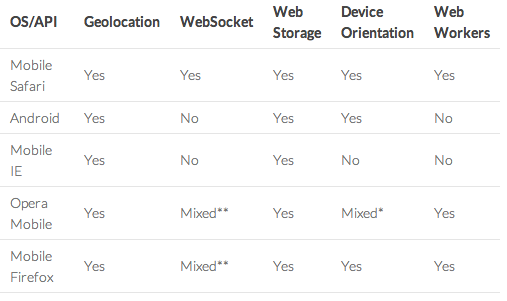
\includegraphics[width=0.8\textwidth]{figuren/html5e}
  \caption{HTML5e mobiele ondersteuning~\cite{Hales2012}}
  \label{fig:html5e}
\end{figure}

\subsection{CSS3}
\label{ref:css3}
Hand in hand met HTML5 gaat CSS3, dat zorgt voor de presentatie. Het is namelijk het hart van webdesign. CSS3 heeft hetzelfde probleem zoals HTML5 als het aankomt op de ondersteuning bij browsers~\cite{MacDonald2011}. Ook hier is er dus een brede waaier aan kenmerken die nog niet overal worden ondersteund. Kenmerken die enkel in een bepaalde browser ondersteund worden, worden voorafgaan door een browserprefix (zoals \code{-webkit-} voor WebKit gebaseerde browsers en \code{-o-} voor Opera).

In deze sectie zullen we kort belangrijke eigenschappen bespreken zoals \term{media queries}, effecten en lettertypes aan de hand van~\cite{MacDonald2011}.

\subsubsection{Media queries}
Zoals al aangehaald, hebben we verschillende apparaten met verschillende schermen en resoluties. Een goeie webpagina bestaat erin deze elementen zo goed mogelijk te benutten. Dit kan vanaf nu door gebruik te maken van \term{media queries} in CSS3. De website kan zich hiermee aanpassen aan het apparaat waarop het wordt getoond. Dit wordt in het Engels omschreven als \term{responsive design}.
% TODO nederlands woord voor responsive design

Ook CSS3 volgt het principe van achterwaartse compatibiliteit. Browsers die deze \term{media queries} niet ondersteunen, zullen deze negeren en enkel de gewone lay-out toepassen ongeacht het toestel.

\subsubsection{Effecten}
Transparantie, afgeronde hoeken, schaduw en kleurenverloop zijn maar enkele van de nieuwe kenmerken in CSS3. Voorheen moest de webdesigner deze dingen vaak met afbeeldingen oplossen, maar nu kan dit allemaal gebeuren met CSS3. Daarnaast hebben we ook effecten als transformaties en transities. Zo is het mogelijk wanneer men over een afbeelding gaat, deze ingezoomd en geroteerd kan worden. 

Dit is zeer vooruitstrevend om wille van twee zaken. Enerzijds schrijf men dingen makkelijker in CSS dan met JavaScript-code. Anderzijds komt er ook meer en meer ondersteuning vanuit de hardware. Zo worden 3D transformaties in CSS3 versneld door de \term{graphics processing unit} (GPU)~\cite{Hales2012,Kool2012}.

\subsubsection{Lettertypes}
Een laatste kenmerk in CSS3 is de betere ondersteuning van lettertypes. Waar vroeger enkel gewerkt kon worden met veilige lettertypes voor het web, is het nu mogelijk om eigen lettertypes op te laden en te gebruiken op je website.

\subsection{JavaScript}
\label{ref:javascript}
JavaScript gaat terug tot in 1995, toen LiveScript~\cite{McFarland2011}. Het heeft een lange weg afgelegd tot nu en is niet altijd even ernstig genomen. Dit kwam omdat men niet inzag wat er allemaal mee kon worden gedaan. 

Op dit moment is het maar al te duidelijk waar JavaScript in uitblinkt: het aanpassen van het \term{document object model} of kortweg DOM~\cite{PhilDutson2012}. Dit is een API voor HTML-documenten~\cite{Hegaret2004}. Hierdoor kunnen dynamische interfaces gecreëerd worden, kan op gebeurtenissen - zoals ergens op klikken - onmiddellijk gereageerd worden en is de website dan ook meer bruikbaar geworden door deze directe feedback~\cite{McFarland2011}.

% TODO referentie verschillende manieren intrepeteren
Het schrijven van JavaScript is niet gemakkelijk om twee redenen~\cite{McFarland2011}. Ten eerste, vergelijkbaar met HTML5 en CSS3, kunnen browsers JavaScript op verschillende manieren interpreteren. Gelukkig is er de laatste tijd veel gestandaardiseerd, maar toch blijven er nog verschillen. %TODO Sander: is dit niet wat vaag?  `veel gestandardiseerd'.  Concreet maken met referentie?
De ontwikkelaar dient dus tijdens het programmeren met deze verschillen rekening te houden. Ten tweede vergt het schrijven van simpele, veel voorkomende taken soms veel code.

Een oplossing voor de bovenstaande pijnpunten is gebruik maken van een bibliotheek. Een voorbeeld hiervan is de populaire jQuery Core bibliotheek. Het is ook mogelijk om jQuery uit te breiden met verscheidene plug-ins om de functionaliteit nog te vergroten~\cite{McFarland2011}.

%%%%%%%%%%%%%%%%%%%%%%%%%%%%%%%%%%%%%%%%%%%%%%%%%%%%%%%%%%%%%%%%%%
%%%%%%%%%%%%%%%%%%%%%%%%%%%%%%%%%%%%%%%%%%%%%%%%%%%%%%%%%%%%%%%%%%

\section{Mobiele HTML5 raamwerken}
\label{sec:mobiele-html5-raamwerken}
%TODO Sander:  deze sectie slechts alle frameworks aanhalen (ook diegene dat we niet gaan vergelijken).  In een ander hoofdstuk (analyse?) de gebruikte frameworks grondiger bestuderen en argumenteren waarom deze gekozen hebben.  Of waarom we de andere niet gekozen hebben.
In deze sectie gaan we inzoomen op bestaande mobiele HTML5 raamwerken die gebruik maken van de laatste nieuwe technologieën zoals HTML5, CSS3 en JavaScript. Deze raamwerken worden gecategoriseerd volgens twee courante aanpakken~\cite{Oeflman2011}: opmaak-up gedreven en JavaScript gedreven. Bij een opmaak-up gedreven aanpak wordt de webapplicatie voornamelijk in HTML code geschreven. Daarentegen wordt bij een JavaScript gedreven aanpak hoofdzakelijk in JavaScript geprogrammeerd.

\subsection{jQuery Mobile}
jQuery Mobile is een mobiel HTML5 \term{user interface} (UI) raamwerk dat werd aangekondigd in 2010~\cite{Resig2010}. In november 2011 werd versie 1.0 uitgebracht~\cite{Parker2011} en een jaar later werd in oktober versie 1.2 uitgebracht~\cite{Parker2012}. Op het moment van schrijven werkt jQuery Mobile aan versie 1.3~\cite{Parker2012a}. Het raamwerk wordt beheerd door het jQuery Project dat onder andere jQuery Core beheert en waar jQuery Mobile afhankelijk van is~\cite{JQuery2012}. jQuery Mobile wordt door onder andere Adobe, BlackBerry en Mozilla gesponsord~\cite{JQuery2012a}.

\subsubsection{Omkadering}
\paragraph{Programmeertaal}
Om met jQuery Mobile aan de slag te kunnen, heb je niets meer nodig dan kennis over HTML, CSS en JavaScript. Alle UI elementen worden geschreven in HTML en aangeduid met \code{data-}* attributen.

\paragraph{Tools}
Een basis teksteditor voldoet om met jQuery Mobile aan de slag te kunnen. Natuurlijk kan het gemakkelijk zijn om van \term{integrated development environments}~(IDE's) zoals Aptana Studio~\cite{Aptana2012} of WebStorm~\cite{JetBrains2012} gebruik te maken, waardoor je handige kenmerken krijgt zoals \term{code completion}.

Je kan ook gebruiken maken van Codiqua om via \term{drag-and-drop} UI elementen op je scherm te slepen. Codiqua zal automatisch op de achtergrond de HTML code voorzien~\cite{Sperry2012}.

\paragraph{Documentatie}
Documentatie is te vinden op \url{www.jquerymobile.com/demos/1.2.0}. Hierop is een catalogus te vinden van alle mogelijke elementen waarover jQuery Mobile beschikt. Door de broncode van een voorbeeld te bekijken, kan je zien welke code je moet schrijven om tot dat resultaat te komen.

Naast de UI elementen is er ook documentatie over de API. Deze gaat over initiële configuraties, events en methodes die kunnen worden gebruikt.

% \paragraph{Community}
% Met 7.400 volgers op GitHub~\cite{GitHub2012} en 11.200 volgers op Twitter~\cite{Twitter2012} komt de grote kracht van jQuery Mobile van zijn community . Dit heeft grotendeels te maken met het feit dat jQuery Mobile geniet van het succes van jQuery, dat ook zeer populair is~\cite{Hales2012}.
%TODO Sander: dit komt in de vergelijkingscriteria

\paragraph{Marktadoptatie}
Als we kijken op de website van jQuery Mobile zien we een reeks applicaties gemaakt met hun raamwerk. Enkele voorbeelden zijn webapplicaties voor Ikea, Disney World, Stanford University en Moulin Rouge~\cite{JQuery2012a}. 

\paragraph{Licenties}
Vanaf september 2012 is het enkel nog mogelijk om jQuery Mobile onder de Massachusetts Institute of Technology (MIT) licentie te verkrijgen~\cite{Dmethvin2012}. Dit betekent dat de code wordt vrijgegeven als \term{open-source} en dat deze tegelijkertijd kan worden gebruikt in propriëtaire projecten en applicaties~\cite{PhilDutson2012}.

\subsubsection{Code en ontwikkeling}
Zoals werd aangehaald, schrijft men vooral HTML5 code voorzien van \code{data-}* attributen. Daarna zal het raamwerk door middel van \term{progressive enhancement} allerhande code toevoegen om de beoogde UI elementen correct te tonen in de browser. Dit wordt verder uitgelegd in de sectie browserondersteuning (zie \ref{sec:jqm-browser-support}).

Er zijn drie strategieën om webapplicaties te maken in jQuery Mobile~\cite{Broulik2012}. Een eerste is om de volledige applicatie in één webpagina te schrijven. Met andere woorden,  de vele schermen van de webapplicatie zijn dan allemaal samengebracht op eenzelfde webpagina. Het voordeel bij deze aanpak is dat er initieel minder verzoeken zijn naar de server omdat alles in één bestand wordt opgehaald. Dit geldt ook zo voor de geïmporteerde CSS en JavaScript-bestanden. 

Een tweede strategie is om voor ieder scherm een aparte webpagina aan te maken. Het voordeel hierbij is dat de eerste pagina waar de gebruiker op terecht komt, sneller wordt gedownload. Bij iedere navigatie naar een ander scherm, moet dit scherm via AJAX worden opgehaald, waardoor dit vertragend kan werken. 

Een laatste strategie is om een mix tussen beide te maken. Men kan bijvoorbeeld alle schermen die de gebruiker vaak nodig heeft op één webpagina plaatsen. De schermen die de gebruiker zelden nodig heeft, plaats men dan op aparte webpagina's.  

\subsubsection{Functionele kenmerken}
jQuery Mobile is een raamwerk dat voornamelijk UI elementen aanbied, met name pagina's en dialoogvensters, werkbalken, knoppen, inhoud vormgeven, elementen voor formulieren en lijsten~\cite{JQuery2012b}.

\paragraph{Pagina's en dialoogvensters}
De basisstructuur van een pagina bestaat uit een koptekst, inhoud en voettekst. Bij het overgaan naar een andere pagina kan men kiezen uit tien overgangseffecten. Voordat deze overgang gebeurt, zal jQuery Mobile altijd eerst die pagina ophalen via AJAX en inladen in het DOM. Zo kan een soepel overgangseffect worden getoond aan de gebruiker. Daarnaast is het ook mogelijk om gelinkte pagina's op voorhand op te halen. Als laatste biedt jQuery Mobile ook dialoogvensters en pop-ups aan. 

\paragraph{Werkbalken}
Het is mogelijk om zowel knoppen bij de koptekst als bij de voettekst te plaatsen. Bij deze laatste kunnen typisch meer knoppen geplaatst worden, bij de koptekst slechts twee. Daarnaast is het ook mogelijk om navigatiebalken te maken. Aan zowel de werk- als navigatiebalken kunnen iconen worden toegevoegd.

\paragraph{Knoppen}
Het is ook mogelijk om knoppen te plaatsen in het inhoud gedeelde. Ook hier is er terug een variëteit aan mogelijkheden: grote of kleine, met iconen of zonder, gegroepeerd of niet. 

\paragraph{Inhoud vormgeven}
De inhoud van de pagina kan worden vormgegeven door gebruik te maken van een rooster. jQuery Mobile laat roosters tot vijf kolommen toe. Daarnaast zijn er ook nog opklapbare blokken ter beschikking. Als laatste kunnen deze blokken ook samengevoegd worden tot een accordeon. 

\paragraph{Elementen voor formulieren}
jQuery Mobile biedt alle gangbare elementen voor formulieren aan zoals textinvoer, een selectie uit een lijst, een zoekveld, een \term{slider} en een \term{switch}. Het raamwerk verplicht zelf om de \code{<label>}-tag te gebruiken. Zo wordt de applicatie toegankelijker gemaakt voor bijvoorbeeld mensen met een \term{e-reader}.

\paragraph{Lijsten}
Een laatste categorie UI elementen die jQuery Mobile aanbiedt, zijn lijsten. Deze gaan van standaard ongeordende lijsten tot lijsten met alle soorten decoraties als iconen, afbeeldingen, telbubbels en verdelers. Ook is het mogelijk om in deze lijsten te zoeken. Hiervoor dient de gebruiker enkel één data attribuut toe te voegen, waarna het raamwerk de implementatie voorziet. 

\subsubsection{Niet-functionele kenmerken}
\paragraph{Performantie}
Zoals gezegd schrijft de ontwikkelaar HTML5 code met specifieke data attributen en zal het raamwerk daarna de code verder aanvullen. Dit gebeurt enkel op de pagina die de gebruiker op dat moment bekijkt. Dit gaat dus ook op voor een webapplicatie waarbij alle schermen op één webpagina zijn geschreven. Deze webpagina bevat allemaal \code{<div>}-verpakkingen voor ieder scherm. jQuery Mobile zal enkel die \code{<div>} verder aanvullen die op dat moment getoond wordt aan de gebruiker. 

\paragraph{Aanpasbaarheid}
Als je jQuery Mobile \term{out-of-the-box} gebruikt, zit alles al goed qua kleur en design. Je hebt de keuze uit vijf kleurenthema's die je kan toepassen op de gehele applicatie of enkel op bepaalde elementen. Om je applicatie echt te laten onderscheiden van de andere, zal je natuurlijk graag je eigen kleurthema willen toepassen. Hier is jQuery Mobile op voorzien door hun \term{stylesheet} op te delen in twee delen: thema's en structuur. Je kan als ontwikkelaar ook enkel de structuur downloaden en zelf de thema CSS schrijven. Daar dit laatste heel wat inspanning vraagt, hebben de ontwikkelaars van jQuery Mobile ook een tool ter beschikking,  namelijk ThemeRoller~\cite{JQuery2012c}. Hier kan je zeer eenvoudig kleuren slepen naar een voorbeeldapplicatie. Eenmaal tevreden kan je de overeenkomstige \term{stylesheet} downloaden en toevoegen aan je project.

\paragraph{Programmeerbaarheid}
Bij het programmeren in jQuery Mobile wordt geen enkel ontwerppatroon afgedwongen. De code voor de UI elementen wordt tenslotte als HTML5 code geschreven. Voor de echte functionaliteit wordt beroep gedaan op JavaScript en meer bepaald op de jQuery Core bibliotheek. Ook deze dwingt geen ontwerppatroon af.

% TODO deze tekst zal later moeten worden verplaatst
Een ander raamwerk, genaamd The-M-Project~\cite{Panacoda2012}, dwingt het Model-View-Controller (MVC) echter wel af. Met dit raamwerk is het mogelijk om webapplicaties te maken die het jQuery Mobile raamwerk gebruiken. In plaats van HTML5-code te schrijven, zoals dat bij jQuery Mobile gebeurt, schrijft je JavaScript-code. The-M-Project zal dan zelf intern deze JavaScript-code omzetten naar de desbetreffende jQuery Mobile HTML5-code.

\paragraph{Browserondersteuning}
\label{sec:jqm-browser-support}
jQuery Mobile deelt browsers op in drie verschillende klassen: A, B en C~\cite{JQuery2012d}. Hierbij ondersteunt een klasse A browser alles, terwijl een klasse C browser enkel de basis HTML ondersteunt (en dus bijvoorbeeld geen hippe CCS3 overgangen).

Er dient een onderscheid te worden gemaakt tussen de begrippen \emph{progressive enhancement} en \emph{graceful degradation}~\cite{Hens2012}. Het eerste is wat jQuery Mobile toepast, namelijk starten met de basis HTML. Deze code wordt door iedere browser, dus ook deze uit de C klasse, op een goede manier weergegeven. Daarna zal het iteratief elementen toevoegen tot het op een moment komt dat de betreffende browser een bepaald kenmerk niet meer ondersteund.

De tegenhanger is \emph{graceful degradation}. Hierbij wordt eerst een versie ontwikkeld die enkel in de meest recentste browser kan worden getoond. Daarna, als de ontwikkelaar nog tijd heeft, gaat hij \term{fallbacks} implementeren waardoor minder recente browser de applicatie ook kunnen weergeven.
%TODO Sander: is het niet nuttiger om progresive enhancement en graceful degration in Kenmerken detecteren en opvullen te bespreken?  jQuery gebruikt enkel progressive enhancement en kan dan verwijzen naar een vorige sectie..

%%%%%%%%%%%%%%%%%%%%%%%%%%%%%%%%%%%%%%%%%%%%%%%%%%%%%%%%%%%%%%%%%%
%%%%%%%%%%%%%%%%%%%%%%%%%%%%%%%%%%%%%%%%%%%%%%%%%%%%%%%%%%%%%%%%%%

\subsection{Sencha Touch}

Sencha Touch is een relatief verschillend raamwerk in vergelijking met jQuery Mobile.  Het wordt ontwikkeld door Sencha,  een bedrijf dat in 2010 is ontstaan als een samensmelting van Ext JS,  jQuery Touch en Raphaël.  Ext JS is een JavaScript raamwerk voor de ontwikkeling van web applicaties. jQuery Touch is een jQuery plugin voor mobiele web ontwikkeling.  Het steunt op WebKit en voegt \term{touch events} toe aan jQuery.  Raphaël,  ten slotte,  is een JavaScript bibliotheek voor vector tekeningen. Op het moment van schrijven is Sencha Touch aan versie 2.1.1~\cite{Inc.}.  

\subsubsection{Omkadering}
\paragraph{Programmeertaal}
Sencha Touch is JavaScript gedreven dus all functionaliteiten worden in JavaScript geïmplementeerd. Het aanroepen van het raamwerk gebeurt door het invoeren van de Sencha Touch bibliotheek binnen \code{<script>}-elementen.  Alle HTML code wordt bij het bekijken van de pagina gegenereerd.  

\paragraph{Tools}
Naast Sencha Touch levert Sencha nog producten die Sencha Touch uitbreiden of het leven van de ontwikkelaar makkelijker maken.  Deze worden hieronder opgelijst~\cite{Inc.}.  

\subparagraph{Sencha Animator}
Dit is een desktop applicatie om CSS3 animaties te ontwerpen.  Deze animaties worden enkel in WebKit browsers ondersteund.

\subparagraph{Sencha Architect}
Dit is een andere desktop applicatie waarmee je makkelijk een UI kan ontwikkelen met behulp van \term{drag-and-drop} commando's.  

\subparagraph{Sencha GXT}
Sencha GXT is een uitbreiding op Google Web Toolkit (GWT).  De compiler van GWT laat toe applicaties in Java te schrijven en ze te compileren naar geoptimaliseerde,  \term{cross-browser} HTML5 en JavaScript.  Sencha GXT voegt grafieken,  widgets, etc. toe aan GWT.

\subparagraph{Sencha.IO}
Deze uitbreiding zorgt voor \term{cloud} services binnen mobiele applicaties.  

\paragraph{Documentatie}
Alle documentatie voor Sencha Touch 2.1.1 is te vinden op \url{docs.sencha.com/touch/2-0}.  Een zoekfunctie voor objecten,  eigenschappen en methoden is aanwezig om snel zaken op te zoeken.  De meeste functionaliteiten zijn voorzien van codevoorbeelden samen met het resultaat hoe de browser de code rendert.  Verder biedt de Sencha website ook een groot aanbod om Sencha te leren gebruiken \url{www.sencha.com/learn/touch/}.  Hier staan handleidingen,  introductie video etc..

%Door de snelle ontwikkeling van Sencha blijft de documentatie niet altijd up-to-date.  Zo zijn vele methoden verouderd maar staat er geen alternatief vermeld. 
%TODO dit is misschien eerer subjectief?
Een ander handig raadslagwerk is de ‘Kitchen Sink'~\cite{Inc.2013}.  Dit is een webapplicatie,  geschreven in Sencha Touch,  die de belangrijkste functionaliteiten bevat samen met de bijhorende code.  


% \paragraph{Community}
% We kunnen vaststellen dat Sencha over een grote community beschikt.  Met meer dan 2 miljoen ontwikkelaars wereldwijd is Sencha de grootste provider van een open-source web applicatie~\cite{Inc.}.  

\paragraph{Marktadoptatie}
Volgens de Sencha website is 50\% van de Fortune 100 - een lijst van de grootste Amerikaanse bedrijven gerangschikt op jaaromzet - een Sencha klant~\cite{Inc.}.  Enkele van hun grootste klanten zijn CNN,  Samsung,  Cisco en  Visa.

\paragraph{Licenties}
Sencha Touch is gratis binnen een commerciële context waarbij het bedrijf in kwestie de broncode niet deelt voor zijn gebruikers.  Wanneer je dit wel wil doen bestaat er ook een gratis \term{open-source} versie van Sencha Touch.  Deze komt met een GNU GPL v3 \term{open-source} licentie wat wil zeggen dat je de vrijheid hebt om aanpassingen aan de broncode te maken en te verspreiden,  zolang je zelf je code maar gratis verspreid voor alle gebruikers.
  
Voor de ontwikkeling van eigen raamwerken of SDKs betaal je een \term{original equipment manufacturer} (OEM) licentie.  Dit wil zeggen dat bedrijven hun producten gaan verkopen onder hun eigen merk en naam, maar gebruik maken van Sencha.  Omdat het gebruik hiervan per gebruiker verschilt,  worden OEM licenties op maat gemaakt~\cite{Inc.}.

\subsubsection{Code en ontwikkeling}
Zoals reeds vermeld moet alle code in JavaScript worden geschreven en dient één HTML bestand slechts als container om de bestanden in te laden.  Sencha valt dus onder JavaScript gebaseerde raamwerken.  De keuze voor deze aanpak heeft twee belangrijke motivaties.  Enerzijds is Sencha Touch gebouwd op Ext JS,  wat op zich een JavaScript raamwerk is.  Anderzijds zorgt het voor een betere ondersteuning voor toestellen met verschillende resoluties.  Samen met SASS en Compass kan Sencha lay-outs definiëren per device (zie sectie \ref{sec:sencha-aanpasbaarheid}).  De \code{Ext.env.Browser} en \code{Ext.env.OS} eigenschappen en \code{Ext.Viewport.getOrientation} en \code{Ext.feature.has} methoden kunnen de vereisten bepalen en de juiste lay-out kiezen~\cite{JohnEClark2012}.

Om het de ontwikkelaars makkelijker te maken biedt Sencha ook SDK tools aan.  Momenteel bevinden deze zich nog in bèta.  Concreet zijn deze tools commando's voor de terminal die onder andere nieuwe projecten kunnen aanmaken, JavaScript bestanden kunnen optimaliseren maar vooral de webapplicatie kunnen omzetten naar native applicaties voor iOS en Android.

\paragraph{Debugging}
Het debuggen van je code gebeurt voornamelijk in de browser zelf.  Tools als de Safari Web Inspector,  Chrome Developer Tools of Firebug moeten de fouten kunnen opsporen.  De broncode van Sencha Touch kan ook ingeladen worden met \code{sencha-touch-debug.js} als bibliotheek.  Deze versie is niet gecomprimeerd en bevat commentaar en documentatie om makkelijker te zoeken waar in de code de fout zich juist bevond.

\subsubsection{Functionele kenmerken}
Net zoals jQuery Mobile heeft Sencha Touch ook een hele hoop functionaliteiten om eenvoudig UI elementen te genereren.  Sencha Touch bevat alle elementen van de UI als JavaScript objecten.  Net zoals alle objectgerichte programmeertalen maken deze objecten gebruik van een klassesysteem,  iets wat slechts vanaf Sencha Touch 2 werd ingevoerd.  Op die manier kunnen klassen worden gedefinieerd (\code{Ext.define}) en aangemaakt (\code{Ext.create}).  Hierbij is ook overerving mogelijk.  De basisklasse van alle objecten is \code{Ext.Component}.  Componenten kunnen gerenderd worden, zichzelf tonen of verbergen,  centreren op het scherm en zichzelf aan- of uitzetten.   Het aanmaken van componenten kan compacter door het gewenste component als \code{xtype} te definiëren.  

Een andere belangrijke component is \code{Ext.Container}.  Containers kunnen subcomponenten bevatten en een lay-out specifiëren.  Alle componenten krijgen een naam die verwijst naar een namespace.  Dit is handig om conflicten te vermijden tussen je eigen objecten en de standaard objecten van het raamwerk.  

Voor een opsomming van alle raamwerk compontenten verwijzen we naar de documentatie~\cite{Inc.2013a}.

%jQuery subsecties:
%Pagina's en dialoogvensters
%werkbalken
%knoppen
%inhoud vormgeven
%elementen voor formulieren
%lijsten

\paragraph{Model}
Data kan intern worden voorgesteld met models.  Dit is iets wat hoort bij het MVC patroon (zie sectie \ref{sec:sencha-programeerbaarheid}).  Een model specifieert een lijst van velden die bij het model horen waarbij een veld een naam en een type heeft.  Optioneel kunnen validaties bij de velden worden toegevoegd om data consistent te houden.  

\paragraph{Store}
\code{Ext.data.Store} is de klasse om instanties van een model op te slaan.  Een \term{store} wordt voorzien van een \term{proxy}.  Deze kan data aan de client of server zijde opslaan.  Een \term{proxy} voor opslag aan client zijde kan zowel in het RAM geheugen als in de \term{local storage} van de browser opslaan.  Een \term{proxy} voor server opslag kan data verzenden via AJAX (zelfde domein) of JSONP (verschillende domeinen).  Een \term{proxy} kan ook nog voorzien worden van een \term{reader} die aangeeft hoe de ontvangen data gelezen moet worden.

\paragraph{View}
Een \term{view} is de benaming voor objecten die aan de gebruiker kunnen getoond worden.  Een voorbeeld hiervan zijn lijsten,  waar vaak de data van een \term{store} wordt in weergegeven.  Zo'n lijst kan makkelijk gefilterd of gesorteerd worden op basis van velden uit het model.  Hiervoor moeten we \term{filters} of \term{sorters} aan de \term{store} toevoegen.  De lay-out van één lijstitem bepalen kan via een \code{XTemplate}.  Het sjabloon bepaalt de HTML structuur van elk item.  Alle gedefinieerde velden van het model kunnen in de template worden opgeroepen of gemanipuleerd.

\subsubsection{Niet-functionele kenmerken}
\paragraph{Performantie}
In vergelijking met versie 1.1 van Sencha Touch is de performantie gestegen om wille van verschillende factoren.  De introductie van het klasse systeem,  zoals besproken in de vorige sectie,  laat toe objecten dynamisch te laden.  Het grote verschil tussen \code{Ext.define} en \code{Ext.create} is dat objecten enkel in het geheugen worden geladen na creatie.  Het is dus de taak van de programmeur om objecten enkel te construeren wanneer ze nodig zijn.

Verder kwam versie 2.0 met een nieuwe lay-out \term{engine} die vooral het verwisselen van oriëntatie van het toestel versnelde.  Ook een verbetering in performantie op Android toestellen,  voornamelijk bij scrollen en animaties,  werd ingevoerd~\cite{Inc.}.

Een benchmark voor deze verbeteringen zijn de opstarttijden van de Kitchen Sink applicatie.  Het opstarten gebeurde met de verschillende Sencha Touch versies en op verschillende toestellen.  De resultaten zijn terug te vinden op figuur \ref{fig:sencha_performance}.  Op bijna elk toestel blijkt Sencha Touch 2.0 ongeveer één seconde sneller te werken~\cite{SenchaInc.2013}.

\begin{figure}
  \centering
  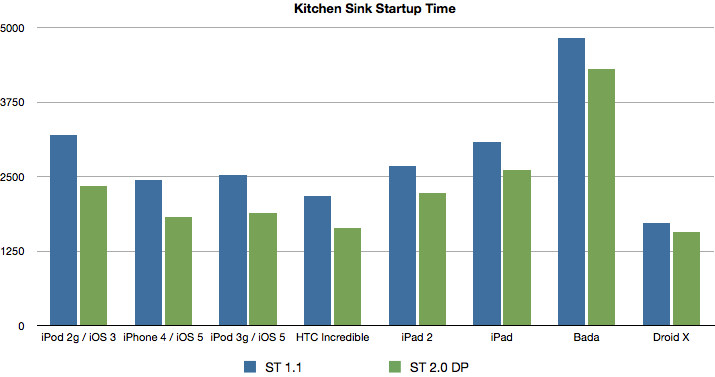
\includegraphics[width=0.8\textwidth]{figuren/sencha-touch-startup-times.png}
  \caption{Sencha Touch Kitchen Sink opstarttijden~\cite{SenchaInc.2013}.}
  \label{fig:sencha_performance}
\end{figure}

\paragraph{Aanpasbaarheid}
\label{sec:sencha-aanpasbaarheid}
Elke component binnen het raamwerk moet overerven van \code{Ext.Component}.  Deze voorziet een attribuut \code{ui}.  De waarde hiervan is een CSS klasse die bepaald hoe de component er zal uitzien.  Sencha heeft al twee CSS klassen voorzien:  \code{light} en \code{dark}.  Andere componenten kunnen deze lijst uitbreiden.  Een knop kan bijvoorbeeld \code{normal},  \code{back},  \code{round},  \code{small},  \code{action} of \code{forward} als \code{ui} waarde hebben.

Het is ook mogelijk om eigen waarden voor \code{ui} te definiëren of de standaarden van Sencha aan te passen.  Hiervoor moet je gebruik maken van SASS en Compass om je CSS bestanden aan te maken.  SASS staat voor Syntactically Awesome Stylesheets en breidt CSS uit met variabelen,  geneste structuren,  mixins en overerving~\cite{Eppstein2013}.  Mixins groeperen enkele CSS eigenschappen en kunnen worden herbruikt.  Compass is een raamwerk bovenop SASS en CSS.  Het compileert SCSS (Sassy CSS) naar CSS bestanden~\cite{Eppstein2013a}.        

Sencha thema's bestaan allemaal uit een set van mixins.  Door zelf mixins te creëren of reeds bestaande te manipuleren kunnen we eigen thema's creëren en ze aan de \code{ui}-waarde van een component toekennen.

\paragraph{Programmeerbaarheid}
\label{sec:sencha-programeerbaarheid}
Zoals reeds aangehaald ondersteund Sencha Touch het MVC (Model-View-Controller) patroon.  Dit patroon vermijdt lange JavaScript bestanden door ze logisch op te delen.  Modellen groeperen velden tot een beschrijving van data-objecten,  views definiëren de weergave van componenten en controllers verbinden beide op basis van events.

In theorie zou het verschil tussen mobiele websites en applicaties enkel in de views terug te vinden zijn.  Echter,  dit wordt nog niet volledig ondersteund en raadt men dus aan om hiervoor aparte projecten te voorzien.

\paragraph{Ondersteuning browser}
Sencha Touch steunt op de WebKit browser \term{engine} dus moet de browser deze bevatten.  Hoewel dit bij de meeste browsers geen probleem meer vormt vallen toch enkele populaire browsers uit de boot.  Sencha Touch is bijvoorbeeld niet compatibel met FireFox Mobile en Opera Mobile~\cite{JohnEClark2012}.

Zoals reeds vermeld zijn er ook methoden voorzien om informatie op te vragen over de context die gehanteerd wordt (browser, OS, toestel, etc.).  Verder kan Sencha Touch ook vragen naar de ondersteuning van specifieke kenmerken (audio,  canvas,  CSS3, …),  analoog als Modernizr.  

Op de Secha website zijn voor sommige browsers en bijhorend besturingssystemen scorecards voorzien om hun compatibiliteit met HTLM5 en Sencha Touch te bespreken~\cite{Inc.}.

%%%%%%%%%%%%%%%%%%%%%%%%%%%%%%%%%%%%%%%%%%%%%%%%%%%%%%%%%%%%%%%%%%
%%%%%%%%%%%%%%%%%%%%%%%%%%%%%%%%%%%%%%%%%%%%%%%%%%%%%%%%%%%%%%%%%%

\section{Vergelijken van raamwerken}
\label{sec:vergelijken-raamwerken}
Om de verschillende mobiele HTML5 raamwerken te kunnen vergelijken hebben we een consistente manier nodig om dit te doen.  Op deze manier worden alle raamwerken op dezelfde manier getest.

\subsection{ISO 25010}
HTML5 raamwerken zijn software en om software te vergelijken bestaat er de ISO 25010 standaard~\cite{Standard2010}.  Hieronder vallen twee modellen:  de productkwaliteit en de kwaliteit van het product in gebruik.  Beide modellen beschrijven de kwaliteit van software op basis van een aantal categorieën met specifieke kwaliteitseigenschappen. Het beoordelen van de categorieën kan gebeuren op basis van een checklist. 

% \begin{figure}
%   \centering
%   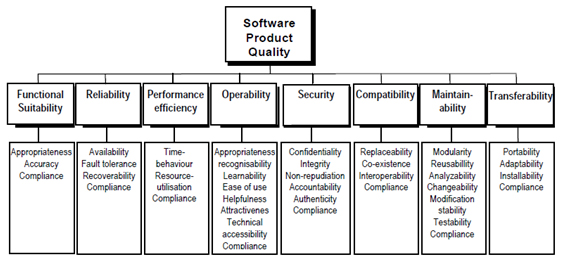
\includegraphics[width=0.8\textwidth]{figuren/iso25010.jpg}
%   \caption{ISO 25010 product kwaliteit model~\cite{Standard2010}.}
%   \label{fig:iso25010}
% \end{figure}
 
\subsubsection{Productkwaliteit}
De acht karakteristieken die horen bij dit model zijn: functionele geschiktheid,  betrouwbaarheid,  performantie, efficiëntie, uitwisselbaarheid,  bruikbaarheid,  betrouwbaarheid, beveiligbaarheid,  onderhoudbaarheid en overdraagbaarheid.   Vanzelfsprekend zijn niet alle categorieën even toepasbaar op HTML5 raamwerken.  Beveiligbaarheid is bijvoorbeeld niet zo belangrijk bij mobiele HTML5 raamwerken.  Performantie en overdraagbaarheid dan weer wel.

\subsubsection{Kwaliteit in gebruik}
De vijf karakteristieken voor dit model zijn: effectiviteit,  efficiëntie,  voldoening,  vrijheid van risico en context dekking. Elke karakteristiek kan toegewezen worden aan verschillende activiteiten van belanghebbenden. Weer zijn alle categorieën niet even toepasbaar.  De risico die een mobiele webapplicatie meebrengt is niet van belang,  het moet vooral efficient zijn en voldoening scheppen.

De kwaliteit voor een systeem in gebruik wordt bepaald door de kwaliteit van de software,  de hardware en het besturingssysteem samen met de gebruikers, hun taken en de sociale omgeving.  De belanghebbenden worden opgedeeld in primaire en secundaire gebruikers.  De eerste zijn de personen die het systeem gebruiken. De laatste zijn diegene die zorgen voor het onderhoud.

\subsection{Bestaande use cases}
Op het web en in de literatuur kunnen we ook \term{use cases} terugvinden waar de proef op de som wordt genomen en twee of meer raamwerken met elkaar worden vergeleken.  Deze werkwijze verschilt van \term{use case} tot \term{use case}

\subsubsection{Codefessions}
Op een blogpost van Codefessions wordt een vergelijking gemaakt tussen jQuery Mobile, Sencha Touch, jQTouch en Kendo UI~\cite{Sarrafi2012}.  Als referentiesysteem gebruiken ze zeven criteria.  De eerste drie zijn de native \term{look-and-feel}, performantie en platform-onafhankelijke capaciteiten.  Deze worden gequoteerd met een cijfer van 0 tot 5 waarbij 5 staat voor de maximale score. Kenmerken worden gequoteerd door de raamwerk met elkaar te vergelijken.  Het raamwerk met de meeste kenmerken krijgt een 5, het tweede beste een 4, enzovoort.  Op een analoge manier wordt code efficiëntie en gebruiksgemak gequoteerd.  Het raamwerk dat de minste lijnen code vereist, krijgt de perfecte score. Hierbij moeten wel alle bestanden gerekend worden die het raamwerk nodig heeft om functioneel te zijn. Licenties krijgen een score van 0 tot 5 waarbij 0 betekent dat het niet beschikbaar is voor een individuele ontwikkelaar en 5 dat het raamwerk \term{open-source} en gratis te gebruiken is. Andere factoren zoals omkadering en uitbreidbaarheid worden niet in de vergelijkingstabel opgenomen omdat ze afhangen van de interesse van de gebruiker.  Ze worden echter wel bekeken.

% \subsubsection{jQuery UI vs Kendo UI}
% Een andere, meer grondige vergelijking is te vinden op \url{www.jqueryuivskendoui.com}~\cite{Bristowe}.  Deze webpagina bestaat uit één grote tabel die meer specifieke kenmerken tussen beide raamwerkenen vergelijkt.  Er worden geen scores uitgedeeld. In de tabel vinden we onder andere een vergelijking van beschikbare thema's,  browser compatibiliteit,  form validatie,  ondersteuning van het product etc.
%TODO meer relevante use cases toevoegen

\subsection{Vergelijkingstabellen}
Naast ISO standaarden of al bestaande use cases, kunnen we ook tabellen raadplegen die zoveel mogelijk raamwerken en zoveel mogelijk kenmerken naast elkaar zetten.  Op Wikipedia creëerde men bijvoorbeeld zo'n tabel voor JavaScript raamwerken~\cite{Wikipedia}.  

Specifiek voor mobiele HTML5 raamwerken bestaat er ook zo'n tabel,  te vinden op \url{www.markus-falk.com/mobile-frameworks-comparison-chart}~\cite{Falk2011}.  We zien er een matrix met als rijen de verschillende raamwerken en in de kolommen de vergelijkingscriteria.  Deze laatste worden opgedeeld in compatibiliteit met het besturingssysteem,  doel van de applicatie,  taal voor ontwikkeling,  hardware interactie,  UI,  licenties en andere.  Deze laatste categorie bevat de criteria of er al-dan-niet een SDK beschikbaar is, encryptie ondersteund wordt en of advertenties worden ondersteund.  Handig hierbij is dat de webpagina een stappenplan voorziet waarin je per categorie al je vereisten moet invullen.  De resultaten zijn dan de raamwerken die compatibel zijn met je vereisten.

%%% Local Variables: 
%%% mode: latex
%%% TeX-master: "masterproef"
%%% End: 
